% ============================================================================
% BORRADOR asistido por IA (15-11-2026). Articulo de la Etapa 2 con el formato del survey
% (Research/Pokemon AI Survey.tex). Para Jose:
%  - Cada numero lleva al lado un comentario "% fuente:" con el archivo del repo de donde sale.
%    Las rutas son relativas a la raiz de BringPredictorVGC. El detalle esta en
%    docs/RESULTADOS_ETAPA2.md y en el anexo de Etapa2_resultados.docx (misma carpeta).
%  - Las secciones de metodologia reusan el survey (Etapa 1) y marcan lo que cambio en la
%    Tabla "Changes since Etapa 1". Las ecuaciones son las del survey.
%  - Las figuras son los PNG de esta carpeta (generar_informe.py los regenera).
%  - No se compilo: en este PC no hay LaTeX. Compilar en Overleaf y revisar.
%  - Reescribir con palabras propias y mantener la declaracion de uso de IA (regla del curso).
% ============================================================================
\documentclass[conference]{IEEEtran}
\IEEEoverridecommandlockouts
\usepackage{cite}
\usepackage{amsmath,amssymb,amsfonts}
\usepackage{graphicx}
\usepackage{textcomp}
\usepackage{xcolor}
\usepackage{booktabs}
\usepackage{array}
\usepackage{url}

\setcounter{topnumber}{3}
\setcounter{bottomnumber}{2}
\setcounter{totalnumber}{4}
\renewcommand{\topfraction}{0.9}
\renewcommand{\bottomfraction}{0.8}
\renewcommand{\textfraction}{0.07}
\renewcommand{\floatpagefraction}{0.7}
\renewcommand{\dbltopfraction}{0.9}
\renewcommand{\dblfloatpagefraction}{0.7}

\begin{document}

\title{The state of ML in Pokémon: the benefits of a bring predictor\\
\large Stage 2: formulation, training and evaluation}

\author{\IEEEauthorblockN{José Ignacio Madriz Ortiz}
\IEEEauthorblockN{Sergio Andrés Zúñiga Castillo}\\
\text{Instituto Tecnológico de Costa Rica}\\
\text{Escuela de Computación}
}

\maketitle

\begin{abstract}
At Team Preview in competitive Pok\'emon VGC, each player sees both six-Pok\'emon teams and commits four of
their own, two of which lead: a choice among 90 alternatives that the literature has not measured in
isolation. We formulate it as a two-step Markov Decision Process with a sparse terminal reward, pretrain a
linear autoregressive policy by behaviour cloning on 4{,}831 human battles with partial labels, and refine it
with REINFORCE and a KL penalty toward the cloned policy, playing battles in a local Pok\'emon Showdown server
with a fixed heuristic battle policy on both sides. On 20 test team pairs never seen in training, evaluated
once with a preregistered rule, the agent wins 59.5\% of 1{,}000 battles per pair against a usage-based
rival (95\% $t$ interval 0.561--0.629, three seeds), clearing the 55\% threshold. It clearly beats random and
usage-based brings, improves marginally over behaviour cloning, and is not distinguishable from a simple
type-matchup heuristic. Whether these brings remain good under a different battle policy is left to the
next stage.
\end{abstract}
% fuente: 4 831 = particion train (docs/EXPERIMENTS.md §2); 0.595 y 0.561--0.629: src/output/tabla_test_vs_usage_argmax.md

\begin{IEEEkeywords}
Pokémon VGC, Reinforcement Learning, Behaviour Cloning, Team Preview, Pokémon Bring
\end{IEEEkeywords}

\section{Introduction}
Stage 1 of this work surveyed fourteen studies on machine learning for competitive Pok\'emon and found the
Team Preview decision effectively unmeasured: most agents play formats without it, VGC-Bench folds it into the
battle policy's action space without isolating it \cite{angliss2026}, and the one system that reports a Team
Preview component publishes no result for it \cite{rodriguez2024}. This paper reports Stage 2: the final
formulation, the training of the agent and its baselines, and the multi-seed evaluation.

\subsection{Research question}
Can a reinforcement-learning policy that sees both full teams select a bring that wins at least 55\% of
battles against a population-usage baseline, when both sides play the battle with the same fixed policy?
The 55\% threshold is the win rate at which the balance literature classifies a strategy as dominant, as
argued in Stage 1.

\section{Methodology}
This section restates the Stage 1 formulation as implemented. Table~\ref{tab:changes} lists every
departure from the Stage 1 proposal and its reason.

\begin{table*}[!t]
\centering
\caption{Changes since the Stage 1 proposal.}
\label{tab:changes}
\footnotesize
\renewcommand{\arraystretch}{1.15}
\begin{tabular}{@{}p{3.6cm}p{4.6cm}p{8.2cm}@{}}
\toprule
\textbf{Element} & \textbf{Implemented} & \textbf{Reason} \\
\midrule
Policy model & Linear autoregressive softmax over hand-crafted per-Pok\'emon features & About 9.7k training examples; closed-form gradients checked by finite differences; numpy only. A Transformer and then DeepSets were planned and dropped. \\
Training regime & Behaviour cloning on logs, then online REINFORCE in Showdown & Logs give $(s,b,R)$ only for brings humans chose; online play gives outcomes for any bring the policy samples. \\
Search baselines and GA & Replaced by an exhaustive planner that maximises $\hat v$ over the 90 brings & With 90 actions, enumeration is exact and cheaper than a genetic algorithm. \\
Usage baseline & Usage without archetype conditioning & Archetype labels are not in the data; species-level usage keeps the baseline reproducible. \\
$\hat v$ embedding $\phi_x$ & Embeddings of species, item, ability and moves through a two-layer MLP ($d=64$, $K=16$) & Same functional form as the survey; the MLP is a project choice. L2 replaces dropout. \\
Seeds and opponents & 3 seeds, one rival (stochastic Usage) & Minimum required by the course; a population of opponents was out of scope. \\
Diagnostics & Lead-pair match and permissive full-bring match & The two most informative of the four planned; per-slot recall and strict full-bring were cut. \\
Exploitability (best response) & Not measured & Out of scope for Stage 2; moved to Stage 3 with a second battle policy. \\
Battle policy $\pi_b$ & \texttt{SimpleHeuristicsPlayer} with automatic Mega Evolution & The original player never Mega Evolves, which would disable a format mechanic. \\
Unknown stat spreads & Imputed by a fixed role-based rule, equal for both sides & Open team sheets omit stat points and natures. \\
\bottomrule
\end{tabular}
\end{table*}
% fuente: Research/ETAPA2_PLAN_v2.md §0 y A9; src/models/bc.py; src/models/vhat.py (docstring); src/baselines/planner.py; src/baselines/usage.py; src/config/arena.yaml (auto_mega, a8_rule); src/utils/spreads.py

\subsection{The problem, abstracted}
Following \cite{angliss2026}, a VGC battle is a two-player, zero-sum, partially observable, stochastic game.
With open team sheets and fixed team configurations $c_1, c_2$ revealed at Team Preview, each player selects a
bring $b_i$: an unordered pair of leads and an unordered pair of reserves from their six Pok\'emon,
\begin{equation}
|\mathcal{B}| = \binom{6}{2}\binom{4}{2} = 15 \times 6 = 90 .
\label{eq:actionspace}
\end{equation}
The learning problem is to find a policy $\rho(b_1 \mid c_1, c_2)$ that maximises the expected terminal reward
when the battle is played by a shared fixed battle policy $\pi_b$, which removes player skill from the evaluation.

\subsection{The decision as a Markov Decision Process}
\label{sec:mdp}
Fixing the rival's bring policy (stochastic Usage) and the battle policy $\pi_b$ for both sides absorbs the
rival into the environment and reduces the game to a single-agent MDP
$\mathcal{M} = \langle \mathcal{S}_{\mathcal{B}}, \mathcal{A}_{\mathcal{B}}, T_{\mathcal{B}}, R_{\mathcal{B}}, \gamma \rangle$
with horizon two, the same device used by \cite{reis2024,reis2025}.

\paragraph{State} $s = \langle c_1, c_2, m, \ell \rangle$: both team sheets, metagame features $m$ computed on
the training window only (per-species rates of being lead, reserve or left out, with fractional counts and
leave-one-out per battle), and the committed lead pair $\ell$, empty at $t=0$. The agent is denied the rival's
bring, the number of revealed Pok\'emon, the battle length, ratings and Bo3 history: the first is simultaneous
and hidden, and the next two are proxies for the outcome.
% fuente: docs/MDP.md (Estado, Informacion que se le niega al agente); src/utils/usage.py

\paragraph{Actions} At $t=0$ the agent commits the lead pair (15 options); at $t=1$, the reserves among the
four remaining (6 options). The composition is the bring, and $15 \times 6 = 90$ as in (\ref{eq:actionspace}).
Factorising lowers the branching per step without changing the set of reachable brings.

\paragraph{Transitions} The first is deterministic ($\ell \leftarrow a_0$). The second plays the full battle in
a local Showdown server under $\pi_b$ for both sides, with the rival's bring sampled from Usage; damage rolls,
accuracy, secondary effects and speed ties make it stochastic.

\paragraph{Reward} Sparse and terminal: $R_{\mathcal{B}}(s,a_0)=0$ and $R_{\mathcal{B}}(s,a_1) \in \{-1,+1\}$,
with $0$ for a draw or a battle past 50 turns, and $\gamma=1$. Stage 1 argued against shaping: the episode is
two decisions long, so there is no credit-assignment gap to bridge, and shaped rewards in this domain have been
exploited \cite{reis2025,karten2026}. No draws or capped battles occurred in test.
% fuente: docs/MDP.md (Recompensa); src/config/arena.yaml (max_turns 50); draws 0 en summary de src/output/arena_*_test_*/meta.json

\subsection{Observability and partial labels}
A log records the two leads of each player exactly, but a reserve only if it entered the field, so the
observation of a logged bring is $o = \langle L, V \rangle$ with $V$ the revealed reserves. Stage 1 measured
84.1\% of player-brings complete, with disclosure correlated to the outcome, so incomplete records are kept,
not filtered. The set of brings consistent with $o$ is
\begin{equation}
\mathcal{C}(o) = \{\, b = (L, R) \;:\; V \subseteq R \subseteq c \setminus L \,\} ,
\label{eq:consistent}
\end{equation}
and behaviour cloning maximises the likelihood of that set,
\begin{equation}
\mathcal{L}_{BC} = -\sum_{o \in \mathcal{D}} \log \sum_{b \in \mathcal{C}(o)} \rho(b \mid s) .
\label{eq:partial}
\end{equation}
The parser that extracts $o$ was checked against 20 training replays annotated by hand (10 per author): both
leads and revealed reserves matched in all 20.
% fuente: src/tests/fixtures/annotated_replays.json; src/tests/test_parser_annotated.py (20 passed)

\subsection{Policy and behaviour cloning}
Each Pok\'emon $x$ in the agent's team is described by a fixed vector $\phi_x$ computed against the full rival
team: train log-rates of being lead, reserve or left out, normalised usage, offensive and defensive type
effectiveness against the six rivals, and a species one-hot (\texttt{<UNK>} if unseen). The policy is
\begin{equation}
\pi_\theta(p,r\mid s)=\operatorname{softmax}_p\Big(\sum_{x\in p}\theta_L^\top\phi_x\Big)\,
\operatorname{softmax}_{r\mid p}\Big(\sum_{x\in r}\theta_R^\top\phi_x\Big),
\end{equation}
with illegal options masked. $\rho_{BC}$ is trained on both sides of every training battle with
(\ref{eq:partial}): Adam ($\eta=0.01$), L2 $10^{-4}$, batch 256, at most 40 epochs with patience 5 on the
validation loss of complete records. Three seeds.
% fuente: src/utils/features.py (docstring); src/models/bc.py; src/config/bc.yaml

\subsection{Reinforcement-learning agent}
The agent starts from $\rho_{BC}$ and minimises
\begin{equation}
\mathcal L(\theta)=-\mathbb E\big[(R-\bar R_{\text{batch}})\log\pi_\theta(b\mid s)\big]
-\beta_H\,\mathcal H[\pi_\theta]+\beta_{KL}\,\mathrm{KL}(\pi_\theta\,\|\,\rho_{BC}) .
\end{equation}
REINFORCE fits the problem: episodes are two steps long with a terminal reward, so the Monte Carlo return is
exact and unbiased and bootstrapped methods (DQN, A2C) add nothing; no replay buffer or target network is used.
The batch-mean baseline reduces variance without a second network. The KL term keeps the policy near human
brings and is meant to limit exploitation of $\pi_b$. Table~\ref{tab:hyper} lists the hyperparameters.

\begin{table}[!t]
\centering
\caption{RL training configuration and budget.}
\label{tab:hyper}
\footnotesize
\begin{tabular}{@{}ll@{}}
\toprule
Optimiser & Adam, $\eta = 0.003$, gradient clip 1.0 \\
Batch & 128 episodes (8 concurrent battles) \\
$\beta_H$ / $\beta_{KL}$ & 0.01 (sweep $\{0, 0.01\}$) / 0.1 \\
Budget & 50{,}048 episodes per seed, 3 seeds \\
Training pairs & 200 train pairs, random side \\
Checkpoint & best validation win rate, every 2{,}000 episodes \\
Hardware & Intel i5-10400F (6 cores), 16 GB RAM, no GPU \\
Wall time per seed & 28--48 min (training 14--26 min) \\
Throughput & 32--61 episodes/s \\
\bottomrule
\end{tabular}
\end{table}
% fuente: src/config/rl.yaml; src/config/arena.yaml (concurrency 8); hardware: docs/EXPERIMENTS.md §7;
% wall time y throughput: wall_time_s (1704-2908 s), train_wall_s (817-1557 s) y T_train_eps_per_s (32.1-61.3)
% en src/output/rl_20261113-141045_s0, rl_20261113-202239_s1, rl_20261114-130136_s2 /meta.json.
% La semilla 0 fue mas lenta (32 ep/s) porque corrio antes del fix de la arena (src/output/FIX_ARENA_REPORT.md).

\subsection{Learned matchup evaluator and baselines}
The evaluator $\hat v$ keeps the bilinear antisymmetric form of Stage 1 \cite{oblander2025},
\begin{equation}
\hat{v}(b_1, b_2) = \sigma\!\left( f(b_1)^{\top} M f(b_2) \right), \qquad M = -M^{\top},
\label{eq:bilinear}
\end{equation}
trained on human logs with the outcome likelihood marginalised over $\mathcal{C}(o_1)\times\mathcal{C}(o_2)$
as in Stage 1. It is only used by the planner baseline, never as the agent's reward, since evaluating with the
function being optimised would be circular. The baselines are:
\begin{itemize}
\item \emph{Random}: uniform over the 90 legal brings (3 sampling seeds).
\item \emph{Usage-argmax}: the most typical bring given train usage rates per species; the literature baseline.
\item \emph{Usage (stochastic)}: softmax of the same score; the rival in every evaluation.
\item \emph{Tipos}: the four Pok\'emon with the best average type matchup against the rival team; the two best lead.
\item \emph{BC}: $\rho_{BC}$ played greedily; the ablation that asks whether RL adds anything.
\item \emph{Planner-$\hat v$}: $\arg\max_{b_1} \sum_{b_2} q_{\text{Usage}}(b_2)\,\hat v(b_1,b_2)$ over the 90 brings.
\end{itemize}
% fuente: docstrings de src/baselines/random.py, usage.py, tipos.py, planner.py; src/models/vhat.py

\subsection{Data and protocol}
We use the Regulation M-A open team sheet logs of \cite{angliss2026} (6{,}902 valid battles of 6{,}905). The
split is temporal and by Bo3 series: train 4{,}831 battles (11-04 to 25-05-2026), validation 1{,}036
(25-05 to 05-06) and test 1{,}035 (05-06 to 20-06). Evaluation uses 10 frozen validation pairs and 20 test
pairs; no team in validation or test appears in train, and test shares no team with validation. Each method
plays the stochastic Usage rival for 1{,}000 battles per test pair (500 per side) and 200 per validation pair.
Per pair we report the win rate; across pairs, the mean over seeds with a $t$ 95\% interval (unit = pair) and
the standard deviation across seeds. The preregistered rule, committed before test, states that the agent
\emph{beats 55\%} only if the lower bound of that interval exceeds 0.55. Test was run once.
% fuente: docs/EXPERIMENTS.md §2, §4, §5 (commit 2e7afb3); src/output/.test_run_done

\section{Results}

\subsection{Main result}
Table~\ref{tab:test} and Fig.~\ref{fig:test} give the test win rates. The agent wins 59.5\% with a lower bound
of 0.561 and therefore beats 55\% under the preregistered rule. The standard deviation across seeds is 0.013.
All 12 evaluations completed with 20{,}000 battles each and no draws or timeouts.

\begin{table}[!t]
\centering
\caption{Test win rate against stochastic Usage (20 unseen pairs, 1{,}000 battles each).}
\label{tab:test}
\footnotesize
\begin{tabular}{@{}lcccc@{}}
\toprule
Method & Seeds & Mean & $t_{95}$ & SD seeds \\
\midrule
RL agent & 3 & \textbf{0.595} & 0.561--0.629 & 0.013 \\
BC & 3 & 0.561 & 0.520--0.603 & 0.012 \\
Tipos & 1 & 0.561 & 0.517--0.606 & -- \\
Usage-argmax & 1 & 0.531 & 0.480--0.581 & -- \\
Planner-$\hat v$ & 1 & 0.506 & 0.463--0.550 & -- \\
Random & 3 & 0.492 & 0.455--0.528 & 0.002 \\
\bottomrule
\end{tabular}
\end{table}
% fuente: src/output/tabla_test_vs_usage_argmax.md (columnas media, t95_bajo, t95_alto, sd_semillas).
% Tipos, Usage-argmax y el planificador son deterministas: una semilla, sin desviacion entre semillas.

\begin{figure}[!t]
\centering
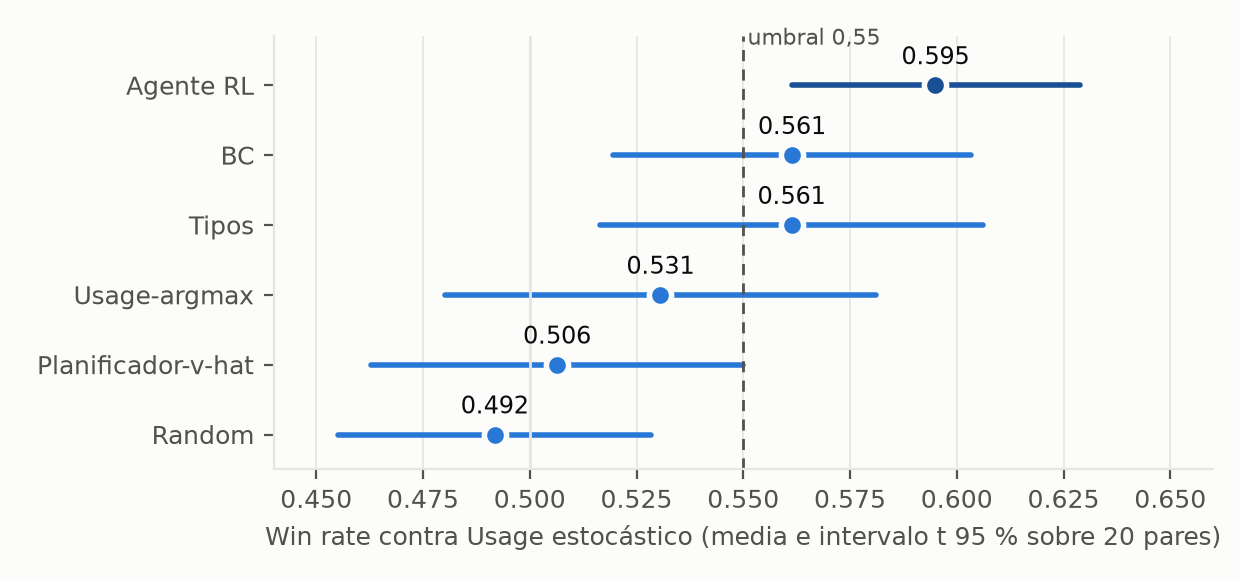
\includegraphics[width=\columnwidth]{fig1_test_winrate.png}
\caption{Test win rate against stochastic Usage: mean over 20 pairs and $t$ 95\% interval. Dashed line: the preregistered 0.55 threshold.}
\label{fig:test}
\end{figure}

\subsection{Paired comparisons}
Table~\ref{tab:diff} and Fig.~\ref{fig:diff} compare the agent with each baseline on the same 20 pairs. The
agent is better than Random and Usage-argmax. Its gain over BC, about 3.4 points, is at the limit of what 20
pairs resolve: the interval only just excludes zero with $1.96\,\mathrm{SE}$ and includes it with a $t_{19}$
multiplier. Against Tipos the difference is compatible with zero, and BC and Tipos are equal
($+0.000 \pm 0.031$). Fig.~\ref{fig:tipos} shows the agent ahead of Tipos on 12 pairs and behind on 8.

\begin{table}[!t]
\centering
\caption{Agent minus reference on the 20 test pairs.}
\label{tab:diff}
\footnotesize
\begin{tabular}{@{}lcc@{}}
\toprule
Reference & Mean $\pm$ SE & 95\% interval ($1.96\,\mathrm{SE}$) \\
\midrule
Random & $+0.103\pm0.024$ & $+0.057$ to $+0.149$ \\
Usage-argmax & $+0.065\pm0.030$ & $+0.006$ to $+0.123$ \\
BC & $+0.034\pm0.017$ & $+0.000$ to $+0.067$ \\
Tipos & $+0.034\pm0.021$ & $-0.007$ to $+0.074$ \\
\bottomrule
\end{tabular}
\end{table}
% fuente: columna dif_vs_<ref> de src/output/tabla_test_vs_{random,usage_argmax,bc,tipos}.md; intervalo = media +- 1.96*EE (docs/EXPERIMENTS.md §4)

\begin{figure}[!t]
\centering
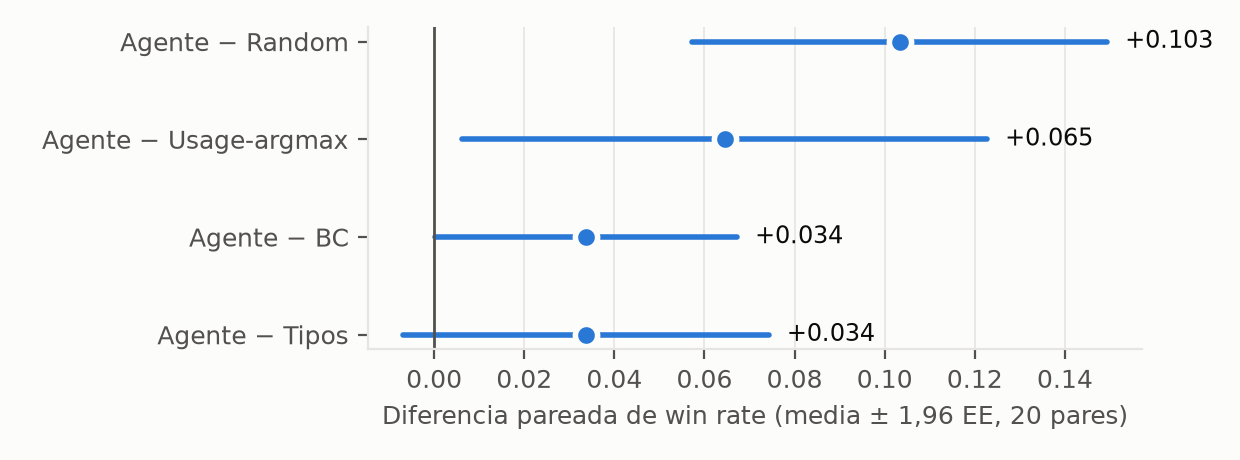
\includegraphics[width=\columnwidth]{fig2_diferencias.png}
\caption{Paired differences, agent minus reference (mean $\pm 1.96\,$SE over 20 pairs).}
\label{fig:diff}
\end{figure}

\begin{figure}[!t]
\centering
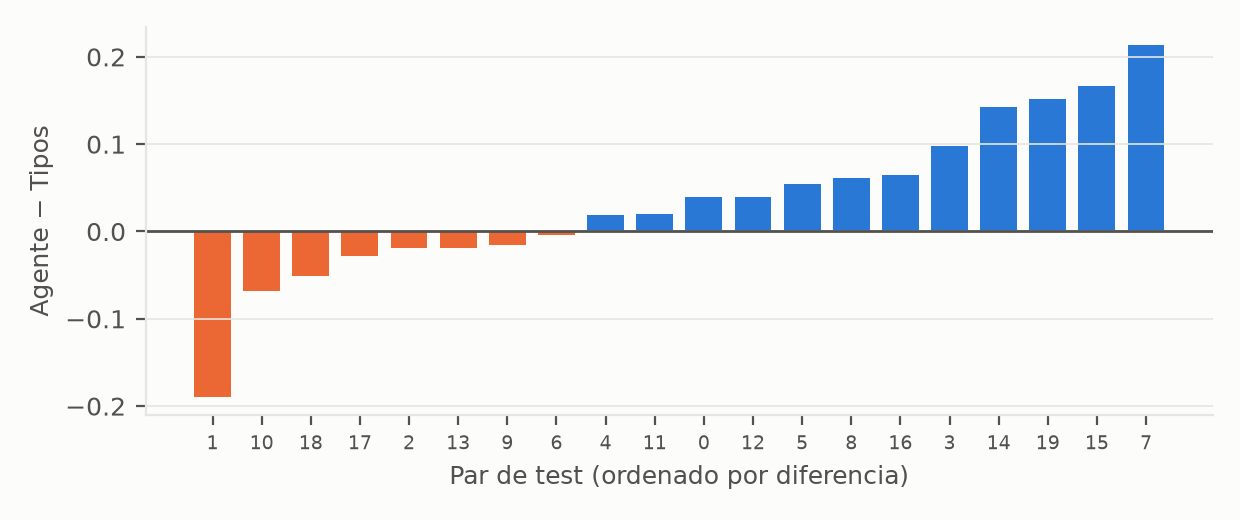
\includegraphics[width=\columnwidth]{fig3_agente_vs_tipos_por_par.png}
\caption{Agent minus Tipos on each test pair (agent averaged over three seeds). Orange: pairs where the agent loses.}
\label{fig:tipos}
\end{figure}
% fuente: per_pair.csv de src/output/arena_agent_vs_usage_test_* (media de 3 semillas) menos arena_tipos_vs_usage_test_20261115-031809_s0

\subsection{Behaviour analysis}

\paragraph{Training curves and exploration} Fig.~\ref{fig:curves} shows validation win rate, policy entropy
and $\mathrm{KL}(\pi_\theta\|\rho_{BC})$ during training for the three seeds with $\beta_H=0.01$ and one seed
with $\beta_H=0$. Validation win rate rises from about 0.50 to 0.60--0.62 in every run. At about 15k episodes,
the same seed reaches 0.539 with $\beta_H=0.01$ and 0.525 with $\beta_H=0$, and the best checkpoints reach
0.616 and 0.623; with a standard error near 0.04 per validation evaluation, neither difference is measurable.
Entropy falls from about 4.2 to 4.0 in both settings, close to the maximum $\ln 90 \approx 4.50$: the entropy
bonus barely matters at this weight, and the policy remains broad while training even though it is evaluated
greedily. The KL grows to 0.09--0.11, so the agent moves only moderately away from the human prior.
% fuente: curves.csv (val_win_rate, entropy, kl_to_bc) de los 4 directorios src/output/rl_*; beta_H en su meta.json;
% EE ~ val_sd_pairs (0.12) / sqrt(10)

\begin{figure*}[!t]
\centering
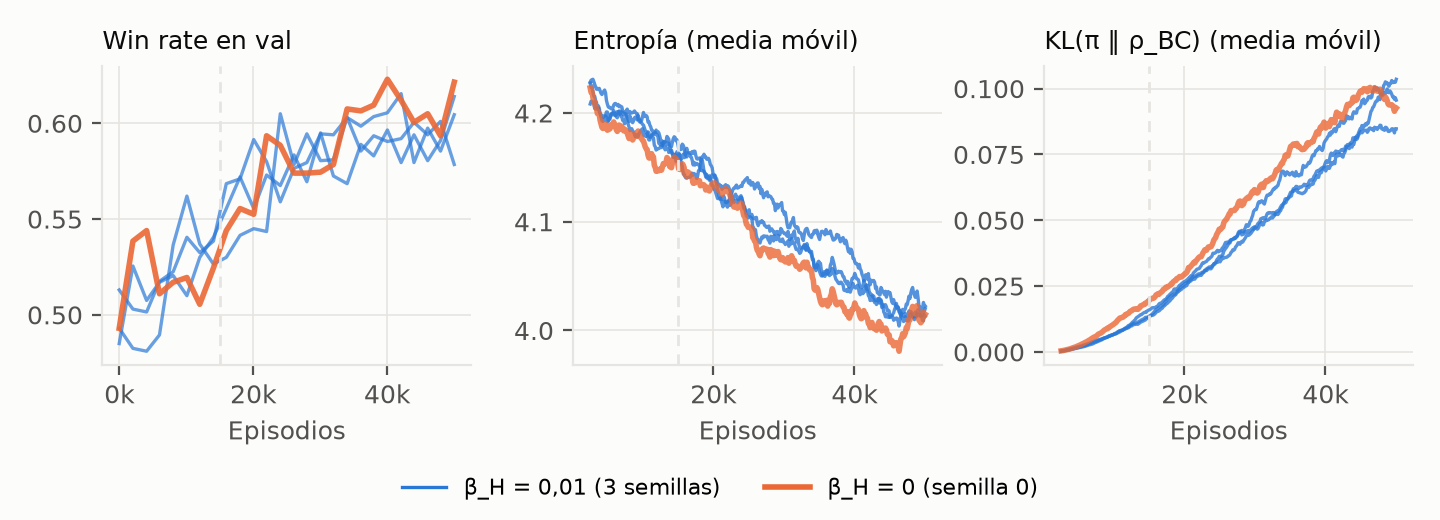
\includegraphics[width=0.85\textwidth]{fig4_curvas.png}
\caption{Training: validation win rate (10 pairs, 200 battles each), policy entropy and KL to $\rho_{BC}$ (moving average over 20 updates). Blue: $\beta_H = 0.01$, three seeds; orange: $\beta_H = 0$, seed 0. Dashed line: 15k episodes.}
\label{fig:curves}
\end{figure*}

\paragraph{Episode length} Battles under $\pi_b$ are short: the median number of turns per pair is 3 to 5 in
test, for every method. Battles this short suggest that the leads decide much of the outcome under the
heuristic player, which may be why a type-matchup heuristic performs as well as the agent; we did not measure
how often reserves enter in the arena battles.
% fuente: columna median_turns de per_pair.csv en src/output/arena_*_test_*

\paragraph{Stability and failure cases} Averaged over pairs the seeds agree closely (SD 0.013), but single
pairs can differ: on pair 0 two seeds win 72\% and the third 49\%, and on pair 1 the seeds win 47\%, 63\% and
42\% while Tipos wins 70\%. Pair 1 is the agent's worst case against Tipos. On pair 6 every method wins
between 47\% and 55\%, so that matchup is hard for all of them. In all 20 pairs the greedy agent uses one bring per side, so these
differences come from which bring each seed converged to, not from sampling.
% fuente: per_pair.csv de arena_agent_vs_usage_test_*_s{0,1,2} y arena_tipos_vs_usage_test_*: win_rate y
% distinct_brings_method (= 2 en todos los pares: un bring por orientacion; 1 en el par 15 de la semilla 2)

\paragraph{Predicting human brings} On 2{,}070 test player-brings, $\rho_{BC}$ predicts the exact lead pair
14.4\% of the time (chance 6.67\%) and a full bring consistent with the observation 4.6\% of the time (chance
1.11\%), with negligible variation across seeds.
% fuente: src/output/diagnosticos_test.json

\paragraph{Validation versus test} On validation, Usage-argmax scored below Random (0.467 vs.\ 0.553), which
suggested that human brings transfer poorly to the heuristic player. On test the order reversed (0.531 vs.\
0.492; Fig.~\ref{fig:valtest}), so the validation result was most likely noise from 10 pairs. Absolute levels
also moved between splits (BC rose from 0.484 to 0.561), which is why the conclusions rest on paired
differences over the same pairs.
% fuente: src/output/tabla_val_vs_usage_argmax.md y tabla_test_vs_usage_argmax.md

\begin{figure}[!t]
\centering
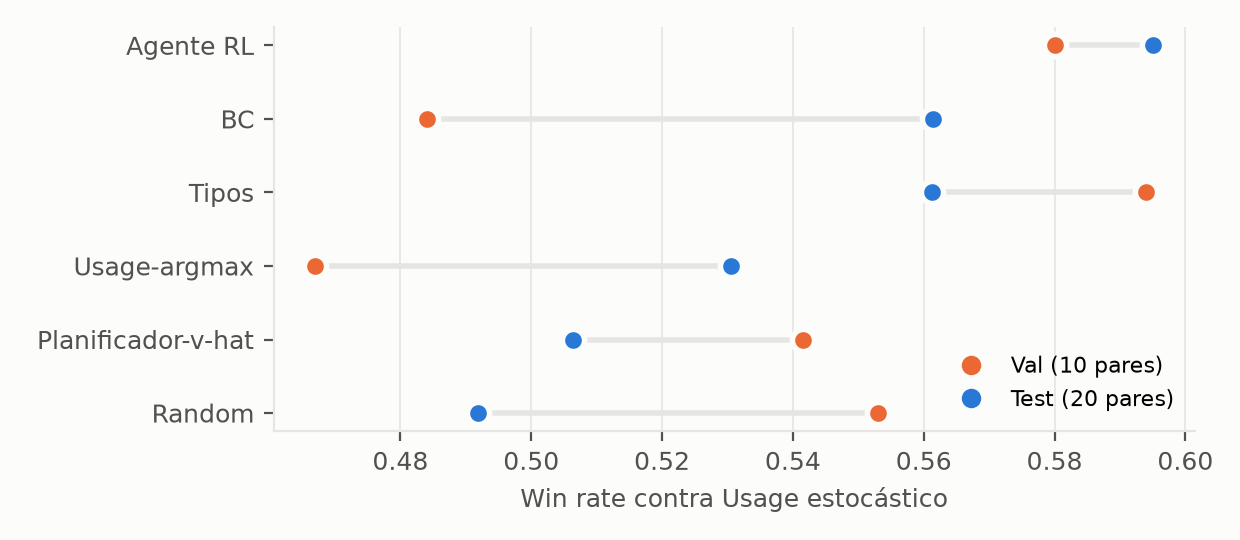
\includegraphics[width=\columnwidth]{fig5_val_vs_test.png}
\caption{Win rate of each method on validation (10 pairs) and test (20 pairs).}
\label{fig:valtest}
\end{figure}

\paragraph{The learned evaluator} The planner falls 5.5 points below BC. With validation accuracy 0.548 and
AUC 0.571, $\hat v$ is too weak to act as a fitness function. These figures are not directly comparable with
the 0.664 accuracy and 0.730 AUC of \cite{oblander2025}, which uses different data, format and labels.
% fuente: dif_vs_bc del planificador en src/output/tabla_test_vs_bc.md; accuracy/AUC de v-hat en val: best_val.val_team_acc
% (0.5483) y val_team_auc (0.5714) en src/output/vhat_20261113-140301_s0/meta.json, el checkpoint que usa el planificador en test.
% Oblander: tabla de src/output/VHAT_PATCH_REPORT.md y el survey.

\section{Discussion and limitations}
The result answers the research question under a strong condition: both sides use the same fixed battle
policy. A bring that wins under $\pi_b$ may exploit its weaknesses instead of being good in human play, and the
KL penalty only partly guards against this. The short battles and the strength of the type heuristic are
consistent with that concern, though they do not prove it. Stage 3 re-evaluates the agent with a second battle policy (MaxBasePower).

Further limitations: a single rival; a linear policy with only additive interactions between Pok\'emon; three
seeds and 20 test pairs; deterministic baselines evaluated once; checkpoint selection on validation; an
exploration sweep with one seed; and diagnostics that measure imitation of human brings, not the quality of
the agent's own brings.

\section{Conclusions}
Under a fixed heuristic battle policy, a REINFORCE agent initialised by behaviour cloning selects brings that
win 59.5\% of battles against a usage-based rival on unseen teams, which meets the preregistered 55\%
threshold. It outperforms random and usage-based brings, improves only marginally over its behaviour-cloning
initialisation, and does not outperform a simple type-matchup heuristic. A learned win-probability model of the
survey's bilinear form was not accurate enough to plan with. The claim that the agent learned good brings,
rather than weaknesses of the heuristic battle player, depends on the Stage 3 evaluation with a second battle
policy.

\section*{Reproducibility}
Code, configuration and results are in the project repository (commits \texttt{2e7afb3}, preregistration, and
\texttt{513505e}, results). The pipeline runs with \texttt{python src/main.py all}, and the final evaluation
with \texttt{python src/main.py test}; Showdown is pinned to commit \texttt{913da36} and poke-env to
\texttt{379a046}. Python 3.14.6, numpy 2.5.4 and pandas 3.1.1; no GPU.
% fuente: requirements.txt; src/main.py (comandos); git log

\section*{Declaration of AI use}
% Mantener: el curso exige declarar el uso de IA. Ajustar al uso real (ver docs/AI_USAGE.md).
An AI assistant (Claude) helped draft code, documentation and parts of this text, under the authors'
direction. The authors chose and justified every design decision, annotated the verification replays by hand,
and reviewed all results reported here.

\begin{thebibliography}{8}

\bibitem{angliss2026}
C.~L. Angliss, J.~Cui, J.~Hu, A.~Rahman, and P.~Stone, ``VGC-Bench: towards mastering diverse team strategies in competitive Pok\'emon,''
in \emph{Proc. 25th Int. Conf. Autonomous Agents and Multiagent Systems (AAMAS)}, Paphos, Cyprus, 2026.

\bibitem{rodriguez2024}
G.~Rodriguez, E.~Villanueva, and J.~Bald\'eon, ``Enhancing Pok\'emon VGC player performance: intelligent agents through deep reinforcement learning and neuroevolution,''
in \emph{HCI in Games}, ser. Lecture Notes in Computer Science, vol.~14730. Cham, Switzerland: Springer, 2024, pp.~275--294.

\bibitem{reis2024}
S.~Reis, R.~Novais, L.~P. Reis, and N.~Lau, ``An adversarial approach for automated Pok\'emon team building and metagame balance,''
\emph{IEEE Transactions on Games}, vol.~16, no.~2, pp.~365--375, Jun.~2024.

\bibitem{reis2025}
S.~Reis, A.~L. Martins, R.~Novais, and F.~Alves, ``A new rules balance track for the Pok\'emon VGC AI competition 2.0,''
in \emph{2025 IEEE Conference on Games (CoG)}, Lisbon, Portugal, 2025, pp.~1--8.

\bibitem{karten2026}
S.~Karten \emph{et al.}, ``The Pok\'eAgent challenge: competitive and long-context learning at scale,''
in \emph{Advances in Neural Information Processing Systems 38 (NeurIPS 2025) Competition Track}, 2025.

\bibitem{oblander2025}
S.~Oblander, ``Representation learning for behavioral analysis of complex competitive decisions,''
Social Science Research Network, Rochester, NY, Working Paper, 2025. [Online]. Available: \url{https://papers.ssrn.com/abstract=4969862}

\end{thebibliography}
% fuente: copiadas tal cual de Research/Pokemon AI Survey.tex. El curso pide BibTeX: cambiar a .bib + IEEEtran.bst antes de entregar.

\end{document}
